\documentclass[]{article}
\usepackage[utf8]{inputenc}
\usepackage{graphicx}
\usepackage{subfig}
\usepackage{euler}

%\usepackage[inner=0cm,outer=0cm,top=0cm,bottom=0cm,paperwidth=10cm,paperheight=3.4cm]{geometry}

\begin{document}

\begin{figure}
\centering
	\subfloat[Top leaflet: POPC]{
		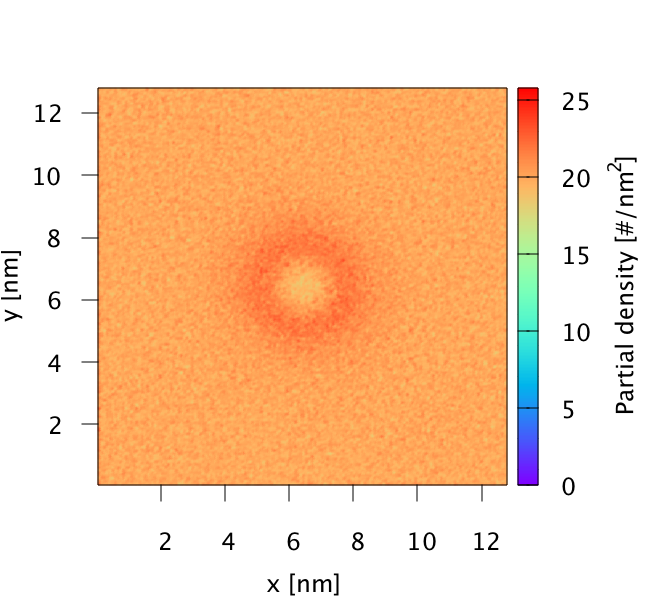
\includegraphics[width=0.5\textwidth]{./up.png}
	}\,%
	\subfloat[Bottom leaflet: POPC]{
		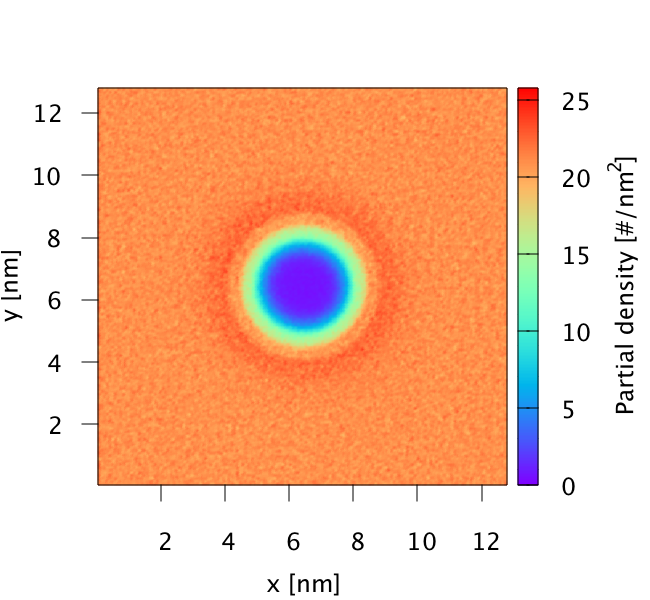
\includegraphics[width=0.5\textwidth]{./down.png}
	}\\%
	\subfloat[Top leaflet: lipid head]{
		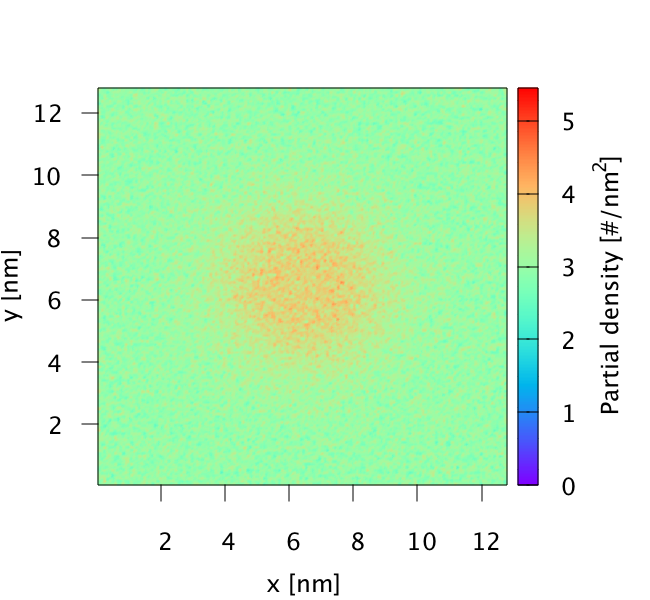
\includegraphics[width=0.5\textwidth]{./NC3PO4Up.png}
	}\,%
	\subfloat[Bottom leaflet: lipid head]{
		\includegraphics[width=0.5\textwidth]{./NC3PO4DOwn.png}
	}\\%
	\subfloat[Top leaflet: lipid tail]{
		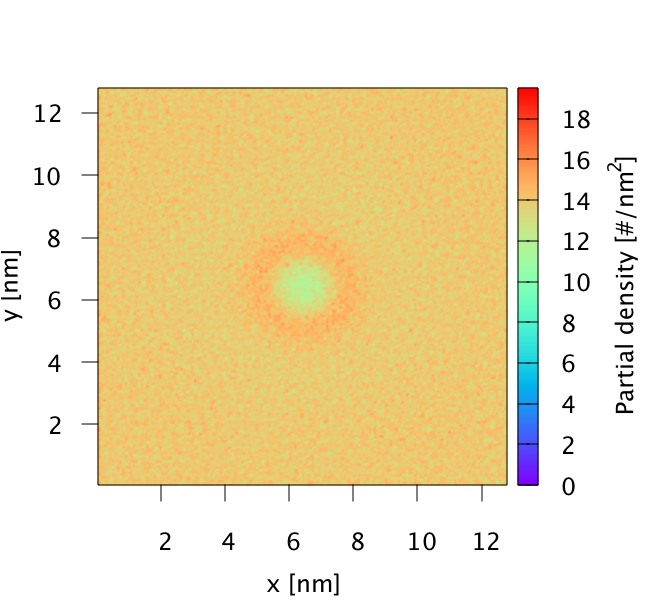
\includegraphics[width=0.5\textwidth]{./tailUp.png}
	}\,%
	\subfloat[Bottom leaflet: lipid tail]{
		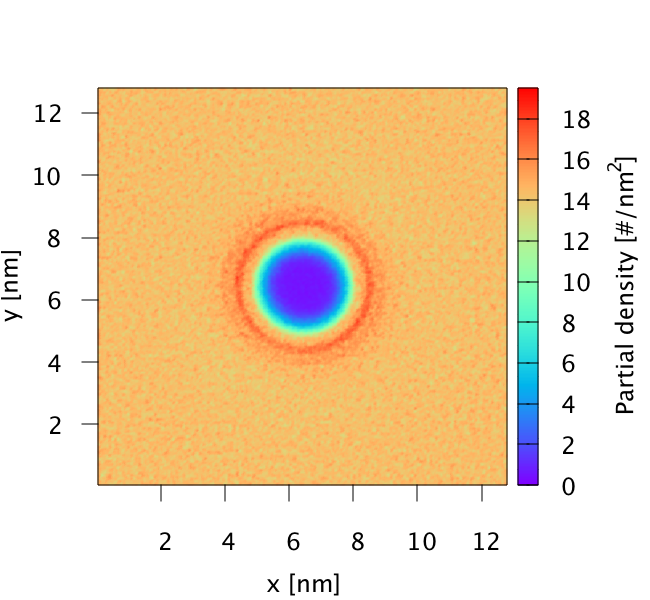
\includegraphics[width=0.5\textwidth]{./tailDown.png}
	}
\end{figure}

\end{document}